\chapter{Bayesian Networks}
Bayesian Networks are a fast and easy way to create graphical models to represent more variables and their relations. \newline
In general \textit{probabilistic graphical models} are graphical representation of the \textit{qualitative}\footnote{The quantitative aspect is represented by the probabilistic distributions.} aspects of probability distributions allowing to:
\begin{itemize}
	\item Visualize the structure of a probabilistic model in a simple and intuitive way, in particular the relations between the variables.
	\item Detect dependency or independency between variables without having to apply derivation rules.
	\item Express complex computations for inference and learning in terms of graphical manipulations.
	\item Represent multiple probability distributions with the same graph, abstracting from their quantitative aspects (e.g. discrete vs continuous distributions).
\end{itemize}
\section{Structure}
A \BN structure $\mathcal{G}$ is directed graph (graphical model).\newline
Each node represents a random variable and each edge represents direct dependency between two random variables, that is one variable that is influenced by the other. This implies also that the father depends on the child, while the second does not depend on the first. \newline
The structure hence can be described as encoding the independences assumptions:
\[
	\mathcal{I}_\ell (\mathcal{G})=\{\forall i~x_i \perp \ND_{x_i}\vert Parents_{x_i}\}
\]
\NDI are all those nodes that are not directly reachable from a node, that is the parents plus all the nodes that are not in its subtree. Let's consider node $x_4$ in Figure~\ref{fig:BayesianNetwork1}, its \NDI are its parents $\{x_1,x_2,x_3\}$ plus $x_5$ which is a non reachable node from $x_4$. In total the \NDI nodes are: $\{x_1, x_2, x_3, x_5\}$
\begin{figure}
	\centering
	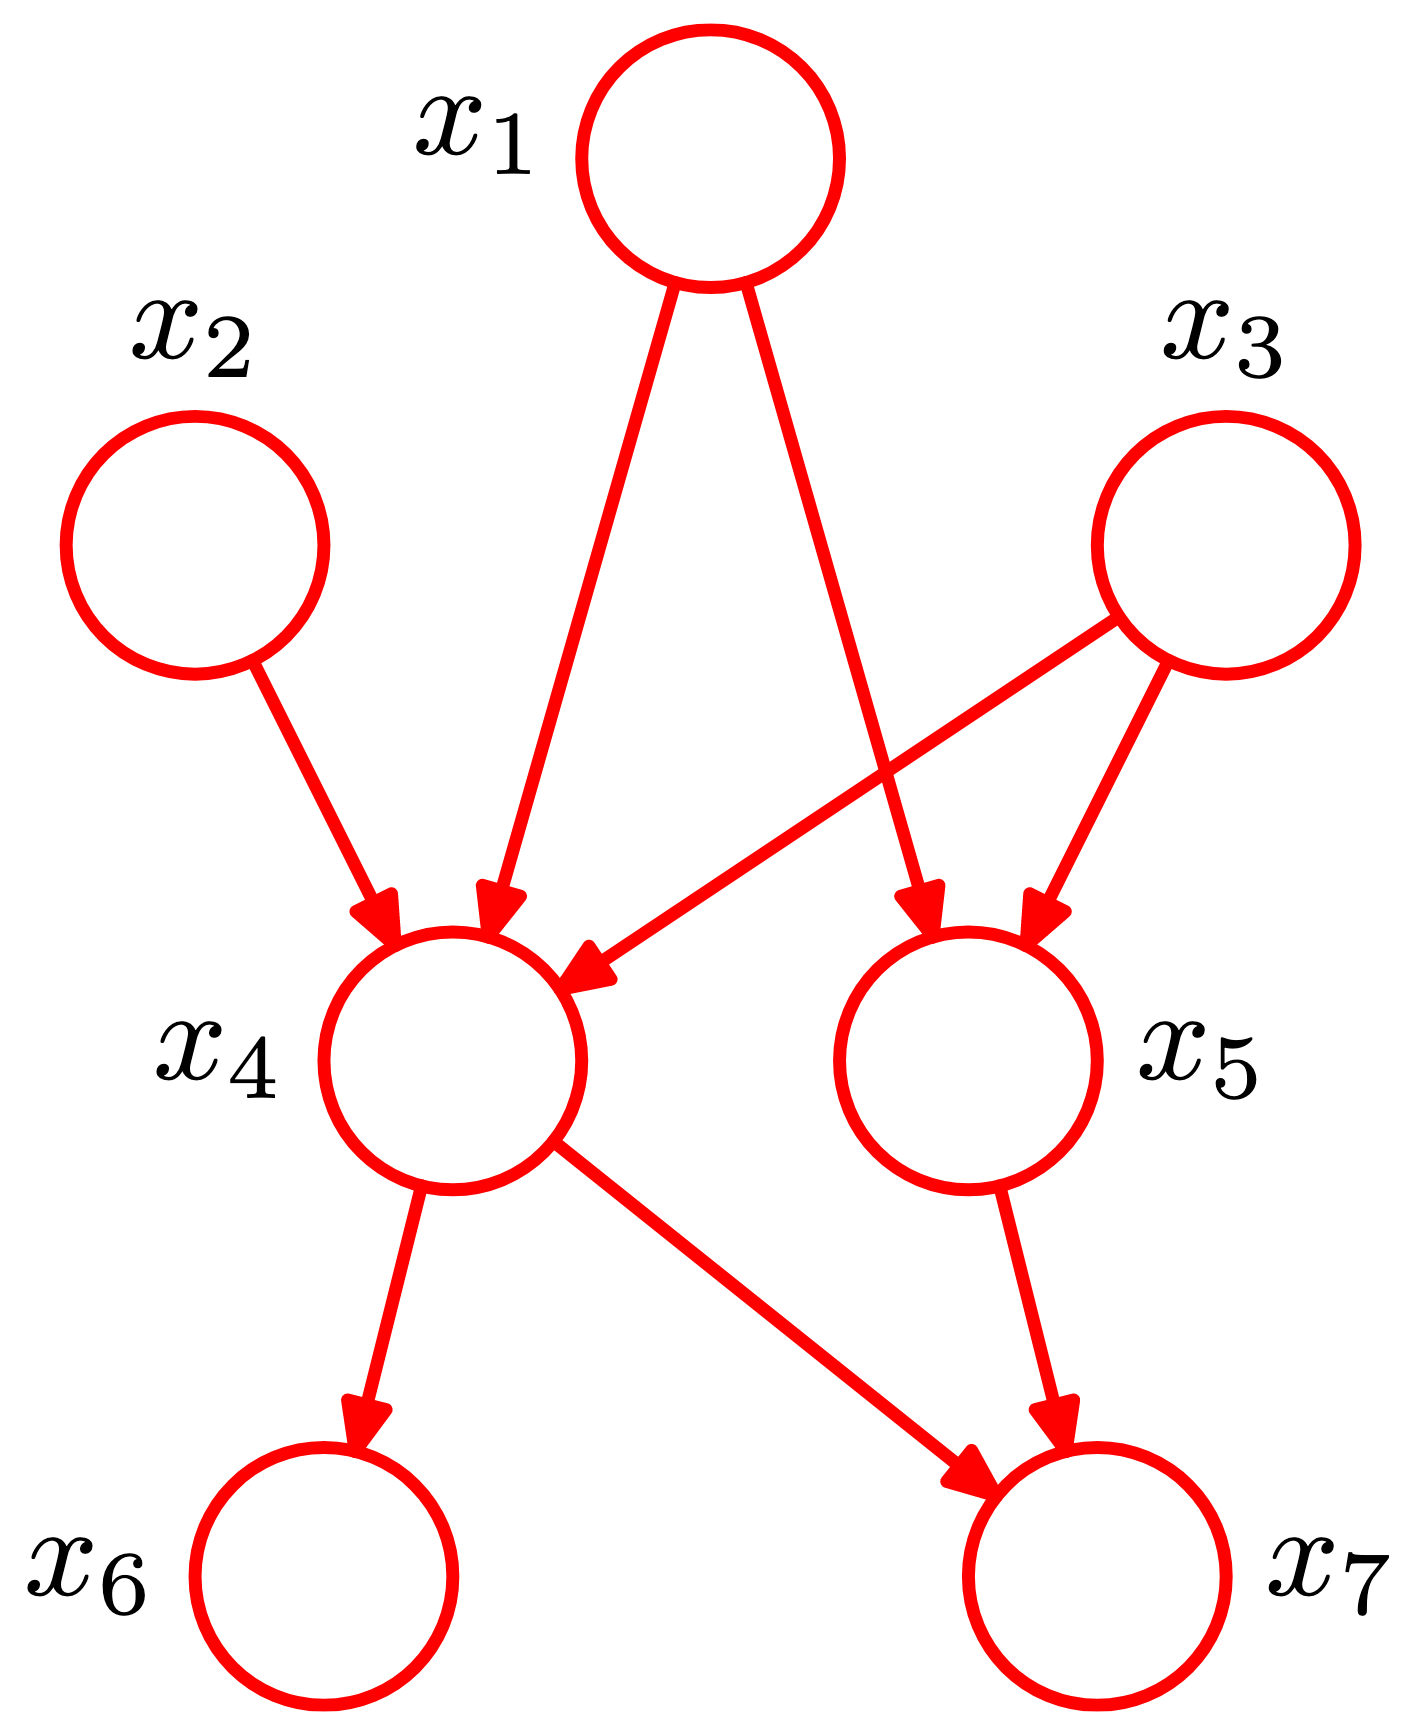
\includegraphics[scale=0.3]{BayesianNetwork1}
	\caption{Example of Bayes Network.}
	\label{fig:BayesianNetwork1}
\end{figure}
The $\mathcal{I}_\ell$ dependency is said to be local (${}_\ell$) since it's defined only wrt to a single variable. \newline
A part from the structure, we need also to have a probability distribution. Let's consider a dataset $\mathcal{D}$ in which all variables are tied with the other by a distribution $p$ which is a joint distribution. We'd like to represent qualitatively with a graph such distribution.\newline
Since the Bayesian Network depends on the independences, it's possible to create a set $\mathcal{I}(p)$ of these by looking at the distribution $p$.\newline
$\mathcal{G}$ is an \textit{independency map} (\textbf{I-map}) for $p$ if $p$ satisfies the local independencies in $\mathcal{G}$:
\[
	\mathcal{I}_\ell(\mathcal{G})\subseteq\mathcal{I}(p)
\]
The sufficient condition for $\mathcal{G}$ to be valid is that all the independences are also in $p$, while the opposite is not always true. Indeed, if some independence from $p$ cannot be modelled into $\mathcal{G}$ via qualitative definition, then they must be modelled quantitatively. \newline
Now we can describe $p$ in terms of the graphical model, that is we can \textbf{factorize} the distribution based on the structure of the model.
\begin{theorem}
$p$ is said to factorize according to $\mathcal{G}$ if:
\begin{equation}
	p(x_1,\hdots,x_m)=\Prod_{i=1}^mp(x_i\vert Parents_{x_i})
	\label{eq:BayesianNetworkFactorization}
\end{equation}
\label{theo:BayesianNetworkFactorization}
\end{theorem}
Mind that this is a double implication: if $\mathcal{G}$ is an I-map for $p$, then $p$ factorizes according to $\mathcal{G}$, then it's true also that if $p$ factorizes according to $\mathcal{G}$, then $\mathcal{G}$ is an I-map for $p$. 
This can be proven as follows.
\begin{proof}
\textit{I-map$\Rightarrow$ factorization}\newline 
If $\mathcal{G}$ is an I-map for $p$, then $p$ satisfies at least these local independences:
\[
\{\forall i~x_i\perp \ND_{x_i}\vert Parents_{x_i} \}
\]
It's possible to order the variable in a topological order relative to $\mathcal{G}$, i.e.:
\[
x_i\rightarrow x_j\Rightarrow i<j
\]
That is the parents have a lower id than the children. Let us now decompose the joint probability using the chain rule as:
\[
p(x_1,\hdots,x_m)=\Prod_{i=1}^mp(x_i\vert x_1,\hdots ,x_{i-1})
\]
Finally local independences imply that for each $x_i$:
\[
p(x_i\vert x_1,\hdots, x_{i-1})=p(x_i\vert Parents_{x_i})
\]
Which by substitution:
\[
p(x_1,\hdots,x_m)=\Prod_{i=1}^m p(x_i\vert Parents_{x_i})
\]
\end{proof}
\noindent Now we need to prove the inverse:
\begin{proof}
Factorization$\Rightarrow$ I-map\newline
If $p$ factorizes according to $\mathcal{G}$, the joint probability can be written as 
\[
p(x_1,\hdots,x_m)=\Prod_{i=1}^mp(x_i\vert Parents_{x_i})
\]
Said $\mathcal{X}$ the set of all variables $x_i$: $\mathcal{X}=\{x_1,\hdots,x_m\}$, let's consider variable $x_m$ (repeat the following steps for the other variable), it's possible to write by the product and sum rules:
\[
p(x_i\vert x_1,\hdots,x_{m-1})=\cfrac{p(x_1,\hdots,x_{m})}{p(x_1,\hdots,x_{m-1})}=\cfrac{p(x_1,\hdots,x_{m})}{\Sum_{x_m}p(x_1,\hdots,x_{m})}
\]
Applying factorisation and isolating the only term containing $x_m$ we get:
\[
	p(x_i\vert x_1,\hdots,x_{m-1})=\cfrac{\Prod_{i=1}^mp(x_i\vert Parents_{x_i})}{\Sum_{x_m}\Prod_{i=1}^mp(x_i\vert Parents_{x_i})}=
\]
\[
	=\cfrac{p(x_m\vert Parents_{x_m})\cancel{\Prod_{i=1}^{m-1}p(x_i\vert Parents_{x_i})}}{\cancel{\Prod_{i=1}^{m-1}p(x_i\vert Parents_{x_i})} \cancel{\Sum_{x_m}p(x_m\vert Parents_{x_m})}}
\]
The sum cancels out because summing all the value of a variable equals to 1. \newline
Hence:
\[
	p(x_i\vert x_1,\hdots,x_{m-1})=p(x_m\vert Parents_{x_m})
\]
\end{proof}
\noindent For example consider Figure~\ref{fig:BayesianNetwork1}. It's possible to write:
\[
	p(x_1,\hdots x_7)=p(x_1)p(x_2)p(x_3)p(x_4\vert x_1,x_2,x_3)p(x_5\vert x_2,x_3)p(x_6\vert x_4)p(x_7\vert x_4,x_5)
\]
Mind that the joint probability $p(x_1, \hdots, x_7)$ is largely influenced by the probability of node 4: $p(x_4\vert x_1, x_2, x_3)$. Now let's suppose that each variable defined a simple binary value, then the total number of possibility would be $2^7$, against the $2^4$ we found right now. This allows to be able to work with a lot of variables. \newline
\begin{definition}[Bayesian Network]
A Bayesian Network is a pair $(\mathcal{G}, p)$ where $p$ factorizes over $\mathcal{G}$ and its represents as a set of conditional probability distribution associated with the nodes of $\mathcal{G}$
\end{definition}
%
%
\subsection{Example}%TODO non so a cosa serva questo esempio
Let's consider another example: genes A and B have independent prior probabilities and gene C can be enhanced by both A and B, with the following probability tables:
\begin{center}
	\begin{tabular}{c|c|cp{2cm}c|c|c}
		Gene&Value&$P(value)$&&Gene&Value&$P(value)$\\
		\cline{1-3}\cline{5-7}
		A&Active&0.3&&B&Active&0.3\\
		A&Inactive&0.7&&B&Inactive&0.7\\
	\end{tabular}
\end{center}
\begin{table}[!h]
	\centering
	\begin{tabular}{cc|cc|cc}
		\multicolumn{2}{c|}{}&\multicolumn{4}{c}{A}\\
		\multicolumn{2}{c|}{}&\multicolumn{2}{c}{Active}&\multicolumn{2}{c}{Inactive}\\
		\hline
		\multicolumn{2}{c|}{}&\multicolumn{2}{c|}{B}&\multicolumn{2}{c}{B}\\
		\multicolumn{2}{c|}{}&Active&Inactive&Active&Inactive\\
		\hline
		C&Active&0.9&0.6&0.7&0.1\\
		C&Inactive&0.1&0.4&0.3&0.9
	\end{tabular}
	\caption{Table showing $p(A,B,\vert C)$.}
\end{table}
%
%
\subsection{Conditional Independence}
First of let's recall Definition~\ref{def:Independence}: two variables $a,b$ are said to be independent written $a\perp b\vert\emptyset$ if: 
\[
p(a,b)=p(a)p(b)
\]
\begin{definition}[Conditional Independence]
Two variables $a,b$ are conditionally independent given $c$, written $a\perp b\vert c$ if:
\[
p(a,b\vert c)=p(a\vert c)p(b\vert c)
\]
\end{definition}
Graphical models allow to directly verify them through the \textbf{d-separation} criterion.
%
%
%
\section{D-separation}
Looking at some simpler graphs, some dependency rules can be inferred and then used on larger graphs by applying them to subgraphs.
%
%
\subsection{Two Nodes}
Given two nodes, or they are independent, hence they are not connected, or they are dependent, hence they are connected.
%
%
\subsection{Three Nodes}
%
\subsubsection{Tail-To-Tail}
Also known as \textit{common cause}.
\begin{center}
	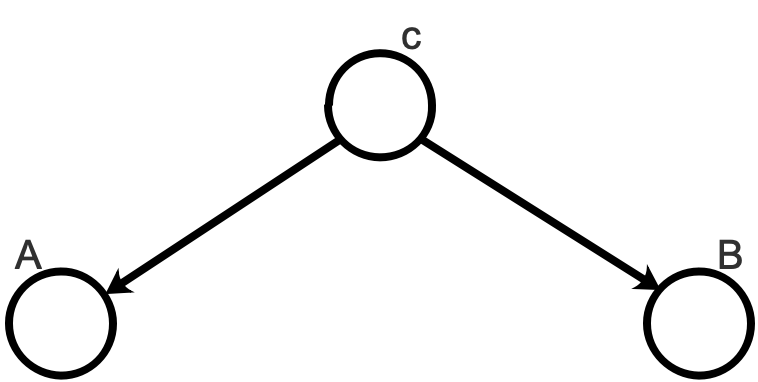
\includegraphics[width=0.4\linewidth]{tailToTailNoGiven}
\end{center}
As for the factorization Equation~\ref{eq:BayesianNetworkFactorization}, the joint distribution can be expressed as:
\[
	p(a,b,c)=p(a\vert c)p(b\vert c)p(c)
\]
The tail-to-tail case says that $a$ and $b$ are \textit{not independent}, written $a \not\!\perp\!\!\!\perp b$. %$a\downmodels b\vert\emptyset$
If $c$ is not given then we have that:
\[
	p(a,b)=\Sum_cp(a\vert c)p(b\vert c)p(c)\neq p(a)p(b)
\] 
On the contrary, if $c$ is given, then they are \textit{conditionally independent}:
\[
p(a,b\vert c)=\cfrac{p(a,b,c)}{p(c)}=p(a\vert c)p(b\vert c)
\] 
\begin{center}
	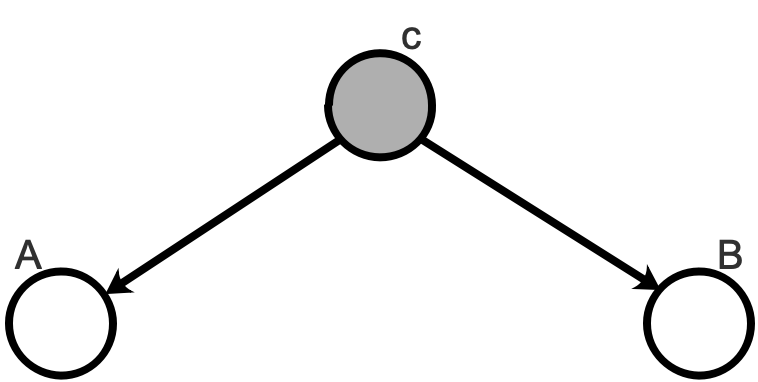
\includegraphics[width=0.4\linewidth]{tailToTailGiven}
\end{center}
Let's consider an example: a company needs to choose the most intelligent ($I$) student between more students. For each student the variables grade $(G)$ and score ($S$) are given. The following graph can be drawn since if the student is intelligent, then it should be seen in both grades and scores. \newline
\begin{minipage}[htp]{\linewidth}
	\begin{minipage}[t]{0.48\linewidth}
		\begin{center}
			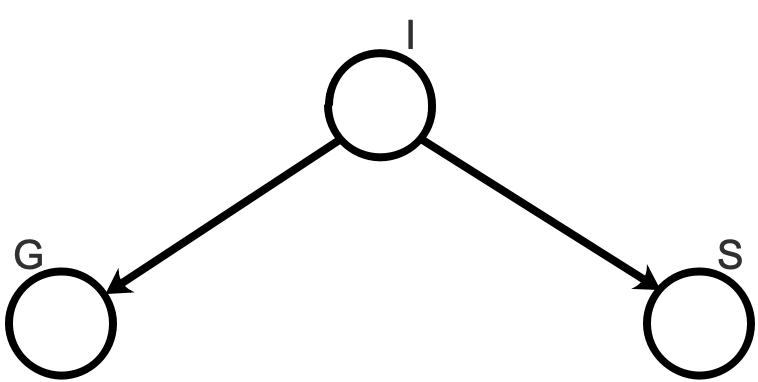
\includegraphics[width=0.7\linewidth]{tailToTailExample1}
		\end{center}
		$G$ and $S$ are directly correlated, for example observing high scores could be indication of having a higher intelligence and hence also higher grades. 
	\end{minipage}
	\hspace{0.04\linewidth}
	\begin{minipage}[t]{0.48\linewidth}
		\begin{center}
			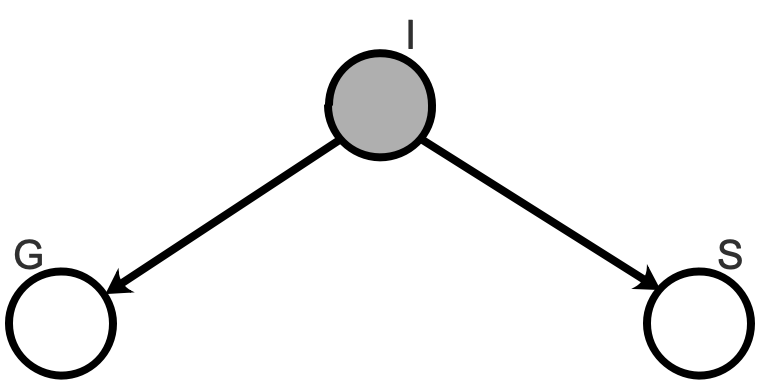
\includegraphics[width=0.7\linewidth]{tailToTailExample2}
		\end{center}
		$G$ and $S$ are not directly dependent since once intelligence has been observed, the correlation disappear and nor $G$ gives more information $S$, nor $S$ gives more information about $G$ than the what we already know. 
	\end{minipage}
\end{minipage}
%
\subsubsection{Head-To-Tail}
Also known as \textit{indirect causal effect}.
\begin{center}
	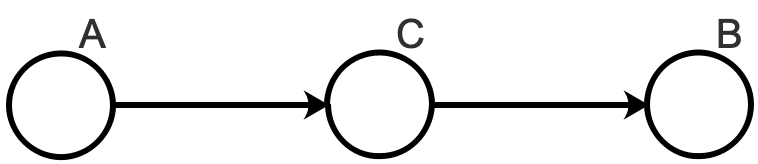
\includegraphics[width=0.4\linewidth]{HeadToTailNoGiven}
\end{center}
The joint distribution can be expressed as:
\[
p(a,b,c)=p(b\vert c)p(c\vert a)p(a)=p(b\vert c)p(a\vert c)p(c)
\]
If $c$ is not given, then then $a$ and $b$ are \textit{not independent}:
\[
p(a,b)=p(a)\Sum_cp(b\vert c)p(c\vert a)\neq p(a)p(b)
\]
If instead $c$ is given, then $a$ and $b$ are conditionally independent:
\[
p(a,b\vert c)=\cfrac{p(b\vert c)p(a\vert c)p(c)}{p(c)}=p(b\vert c)p(a\vert c)
\]
\begin{center}
  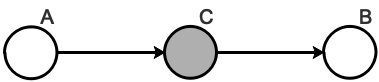
\includegraphics[width=0.4\linewidth]{HeadToTailGiven}
\end{center}
As before, let's consider the example of the intelligence of a student. \newline
\begin{minipage}[htp]{\linewidth}
	\begin{minipage}[t]{0.48\linewidth}
		\begin{center}
			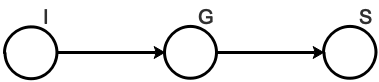
\includegraphics[width=0.7\linewidth]{HeadToTailExample1}
		\end{center}
    Intuitivly, if we observe that the student is intelligent, then we are more inclined to believe that it's grades $G$ are good and that they will have a better score at the interview $S$, that is the probability of these latter events is higher conditioned on the observation that the student is intelligent. 	
	\end{minipage}
	\hspace{0.04\linewidth}
	\begin{minipage}[t]{0.48\linewidth}
		\begin{center}
			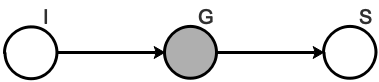
\includegraphics[width=0.7\linewidth]{HeadToTailExample2}
		\end{center}
    Instead if we assume that $G$ is observed, then it's intelligence no longer influences the score of the interview.
	\end{minipage}
\end{minipage}
%
\subsubsection{Head-To-Head}
Also known as \textit{common effect}.
\begin{center}
	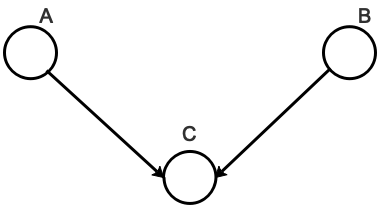
\includegraphics[width=0.4\linewidth]{HeadToHeadNoGiven}  
\end{center}
The joint distribution can be expressed as:
\[
  p(a,b,c)=p(c\vert a, b)p(a)p(b)
\]
If $c$ is not given, then then $a$ and $b$ are \textit{independent}:
\[
  p(a,b)=\Sum_cp(c\vert a, b)p(a)p(b)=p(a)p(b)
\]
If instead $c$ is given, then $a$ and $b$ are not conditionally independent, hence they are conditionally dependent:
\[
p(a,b\vert c)=\cfrac{p(c\vert a,b)p(a)p(b)}{p(c)}\neq p(a\vert c)p(b\vert c)
\]
\begin{center}
  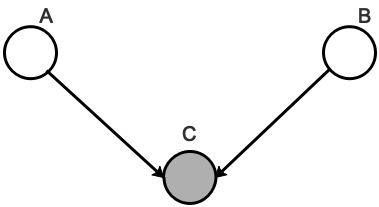
\includegraphics[width=0.4\linewidth]{HeadToHeadGiven}
\end{center}
Let's consider one last time the example of the student that is to be hired from a company. We have said that if $c$ is not given, then $a$ and $b$ are independent, while if $c$ is given they are dependent. Indeed, if $c$ was the score of a test, then the student ($G$) and it was low, we could think that they are actually not that smart, but then if we were to observe that the test was difficult, then we could think that actually they are not \textit{not} intelligent. Hence, $a$ and $b$ are actually correlated if $c$ is given. 
\begin{center}
  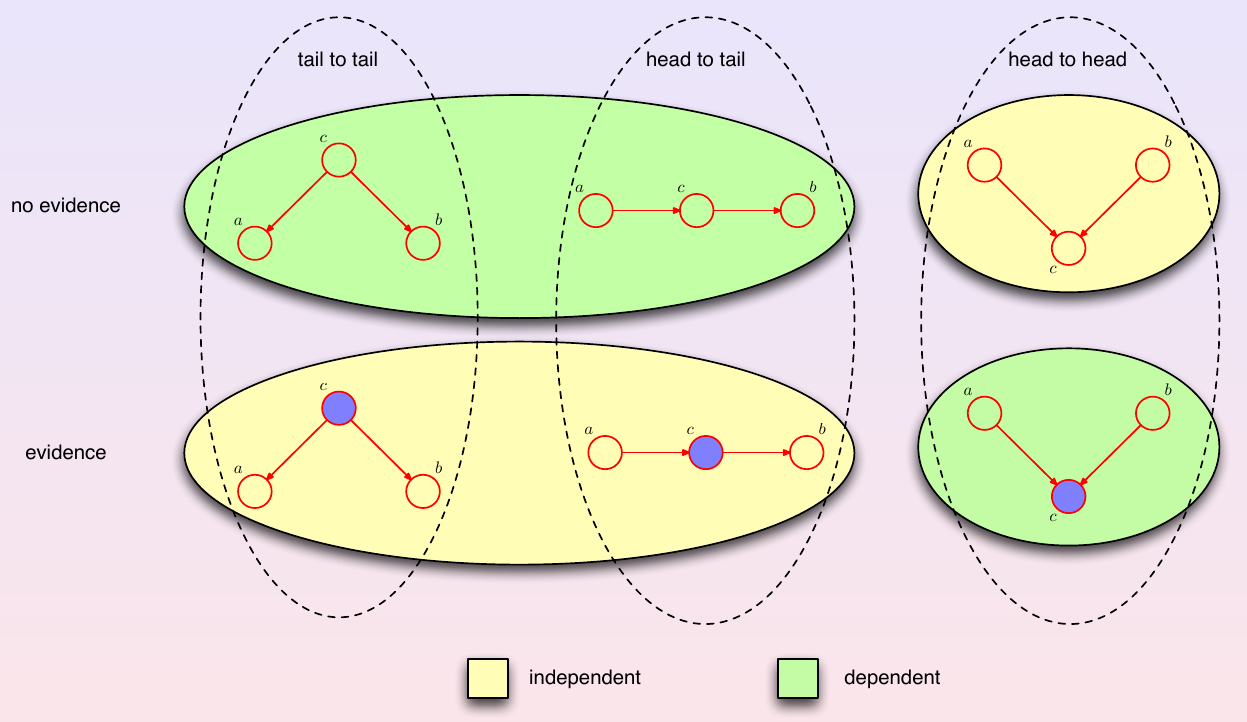
\includegraphics[width=0.8\linewidth]{DSeparationRecap}
\end{center}
\myparagraph{Example Head-To-Head Example}
Let's consider a fuel system of a car. The fuel system is make of:
\begin{itemize}
  \item Battery $B$: can either be charged ($B=1$) or flat ($B=0$);
  \item Fuel tank $F$: can either be full ($F=1$) or empy ($F=0$);
  \item Electric fuel gauge $G$: either full ($G=1$) or empty ($G=0$).
\end{itemize}
Let's now say that the probability of the battery to be charged is $P(B=1)=0.9$ and the probability for the fuel tank to be full is $P(F=1)=0.9$. \newline
The electric fuel gauge is conditioned on both:
\begin{center}
  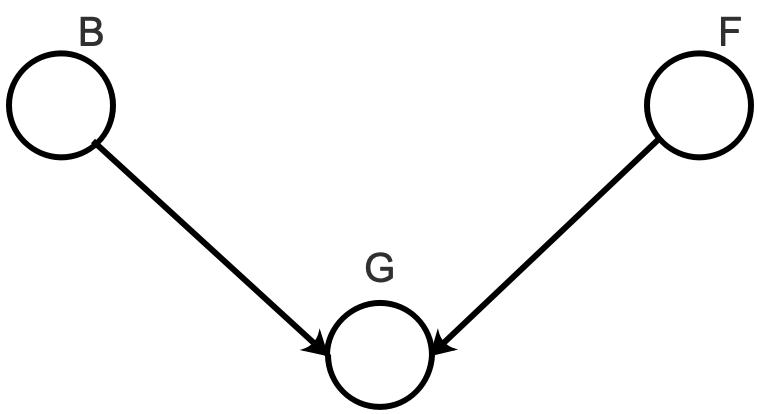
\includegraphics[width=0.5\linewidth]{FuelTankExample1NoGiven}
\end{center}
\[
  \begin{array}{ll}
    P(G=1\vert B=1,F=1)=0.8&P(G=1\vert B=1,F=0)=0.2\\
    P(G=1\vert B=0,F=1)=0.2&P(G=1\vert B=0,F=0)=0.1\\
  \end{array}
\]
We want to compute the probability of having an empty tank:
\[P(F=0)=1-P(F=1)=0.1\]
What would happen to the probability if we were to notice that the fuel gauge was empty? In particular let's compute the probability of the fuel tank to be empty given the fact that the fuel gauge is empty $P(F=0\vert G=0)$. Such probability is not given, hence we need to find it. To compute $P(F=0\vert G=0)$ we could use Bayes:
\[P(F=0\vert G=0)=\dfrac{P(G=0\vert F=0)P(F=0)}{P(G=0)}\]
We need to compute $P(G=0\vert F=0)$ and $P(G=0)$ but they are easier to compute by the product rule:
\[
\begin{array}{ll}
  P(G=0\vert F=0)&=\Sum_{B\in\{0,1\}}P(G=0,B\vert F=0)\\
                 &=\Sum_{B\in\{0,1\}}P(G=0\vert B,F=0)P(B\vert F=0)\\
                 &=\Sum_{B\in\{0,1\}}P(G=0\vert B,F=0)P(B)\\
                 &=P(G=0\vert B=0, F=0)P(B=0)+P(G=0\vert B=1, F=0)P(B=1)\\
                 &=0.9\cdot0.1+0.8\cdot 0.9=0.81
\end{array}
\]
Notice that the passage from the second to the third equation it's possible since $B$ and $F$ are independent, hence $P(B\vert F=0)=P(B)$.\newline 
Similarly $P(G=0)$ is given by:
\[
\begin{array}{ll}
  P(G=0)&=\Sum_{B\in\{0,1\}}\Sum_{F\in\{0,1\}}P(G=0,B,F)\\
        &=\Sum_{B\in\{0,1\}}\Sum_{F\in\{0,1\}}P(G=0\vert B,F)P(B)P(F)=0.315  
\end{array}
\]
In the end it's possible to see that by observing the fact that the fuel gauge is empty, then the probability of the fuel tank of being actually empty increases:
\[P(F=0\vert G=0)=\dfrac{P(G=0\vert F=0)P(F=0)}{P(G=0)}\simeq 0.257\]
Not as much as one would expect, but this is due to strong prior and an unreliable gauge. \newline
Now let's consider the case in which we knew that also the battery is flat. How does the probability $P(F=0\vert G=0,B=0)$ change knowing this information? \newline
It's possible to apply again Bayes Theorem and have:
\[P(F=0\vert G=0, B=0)=\dfrac{P(G=0\vert F=0,B=0)P(F=0\vert B=0)}{P(G=0\vert B=0)}\]
\begin{definition}[Active Trail]
  Let's consider a graph with three node $X,Y,Z$ connected as in one of the cases before. The trail $X\rightleftharpoons Y\rightleftharpoons Z$ is said to be \textit{active} if information can flow from $X$ to $Y$ via $Z$.
  \begin{itemize}
    \item Head-to-Tail $X\rightarrow Z\rightarrow Y$ is active if and only if $Z$ \textbf{is not} observed;
    \item Tail-to-Tail $X\leftarrow Z\rightarrow Y$ is active if and only if $Z$ \textbf{is not} observed;
    \item Head-to-Head $X\rightarrow Z\leftarrow Y$ is active if and only if $Z$ \textbf{is} observed;
  \end{itemize}
\end{definition}
%
%
\subsection{d-Separation -- General Case}
Obviously the majority of the graphs is not made of three nodes, but has many nodes. Suppose that we want to find a path that allows to go from one group nodes holding evidence to another. We can say whether this is possible or not by applying the before rules and by adding the following rule: a head-to-head node $c$ unblocks the dependency path between its parents if either itself or \textit{any of its descendants} receives evidence. \newline
\begin{definition}[Descendant]
  A descendant of a node $x$ is any node which can be reached from $x$ with a path following the direction of the arrows.   
\end{definition}
\begin{theorem}[$d$-Separation General Case]
  Let $\mathcal{G}$ be a Bayesian Network structure and $X_1\rightleftharpoons\hdots\rightleftharpoons X_n$ a trail in $\mathcal{G}$. Let $\vect{Z}$ be a subset of observed variables. The trail $X_1\rightleftharpoons\hdots\rightleftharpoons X_n$ is active given $\vect{Z}$ if:
  \begin{itemize}
    \item Whenever we have a head-to-head structure $X_{i-1}\rightarrow X_i\leftarrow X_{i+1}$, then $X_i$ or one of its descendants are in $\vect{Z}$;
    \item No other node along the trail is in $\vect{Z}$.
  \end{itemize}
\end{theorem}
Note that if $X_1$ or $X_n$ are in $\vect{Z}$, then the trail is not active. \newline
\begin{definition}[Path Blocked]
  A path is said to be blocked if it includes at least one node such that either:
  \begin{itemize}
    \item The arrows on the path meet tail-to-tail or head-to-tail at the node and it is in $C$, or
    \item The arrows on the path meet head-to-head at the node and neither it nor any of its descendants is in $C$. 
  \end{itemize}
\end{definition}
\begin{definition}[General d-separation Criterion]
  Given a generic Bayesian Network and nonintersecting arbitrary sets of nodes $A,B,C$, the sets $A$ and $B$ are d-separated by $C$, written $\dsep{A;B\vert C}$ if all paths from any node in $A$ to any node in $B$ are blocked.
  \label{def:dSeparation}
\end{definition}
Note that d-separation \textit{implies conditional independence}: the sets $A$ and $B$ are independent given $C$, written $A\perp B\vert C$ if they are d-separated by $C$.
%
\subsubsection{Example 1}
Let's consider the following graph:
\begin{center}
  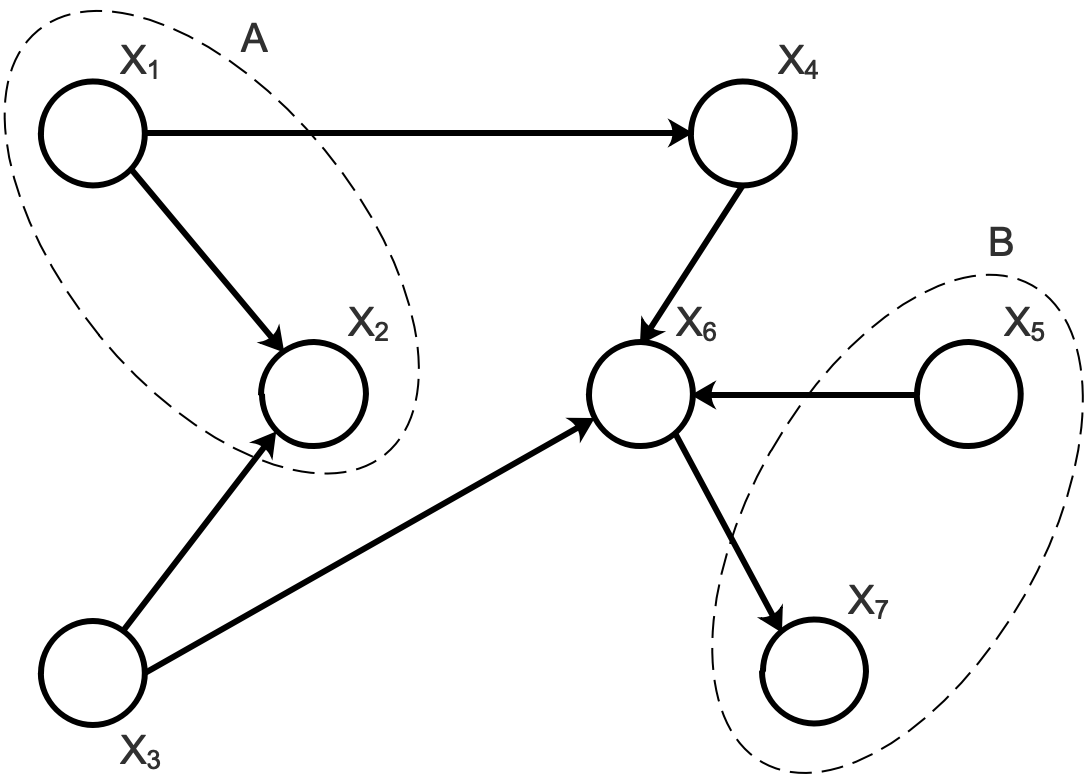
\includegraphics[width=0.7\linewidth]{dSeparationExample1_1}
\end{center}
and three independent sets: $A=\{X_1,X_2\}, B=\{X_5,X_7\}, C=\emptyset$. By applying the rules we need to find a possible path from one set to another. For example let's consider a first possibility made of the path $X_1\rightarrow X_4\rightarrow X_6\leftarrow x_5$: the first three nodes are in a head-to-tail structure, we do not have any information regarding $X_4$, hence the path is active till this point. $X_4\rightarrow X_6\leftarrow X_5$ is a head-to-head structure and there is no evidence on $X_6$, hence the path is blocked. \newline
Let's instead consider the path: $X_1\rightarrow X_4\rightarrow X_6\rightarrow X_7$. We saw that the first three nodes are in a head-to-tail structure and there is no evidence, so the trail is active. Let's then look at the last three nodes: $X_4\rightarrow X_6\rightarrow X_7$: this is head-to-tail structure and there is no evidence on $X_6$, hence the trail is active and an actual path from the set $A$ to the set $B$ could be found. \newline
It's possible to find also a path starting from $X_2$: $X_2\leftarrow X_3\rightarrow X_6 \rightarrow X_7$ which actually works because the first three nodes are in a tail-to-tail structure and there is no evidence on $X_3$, hence the trail is active, and the last three nodes are in a head-to-tail structure with no evidence on $X_6$. \newline
Similarly to before, the path $X_2\leftarrow X_3\rightarrow X_6\rightarrow X_5$ does not work because the last three nodes are in a head-to-head structure and there is no evidence on $X_6$.
%
\subsubsection{Example 2}
Let's consider the case in which $X_6$ is given evidence:
\begin{center}
  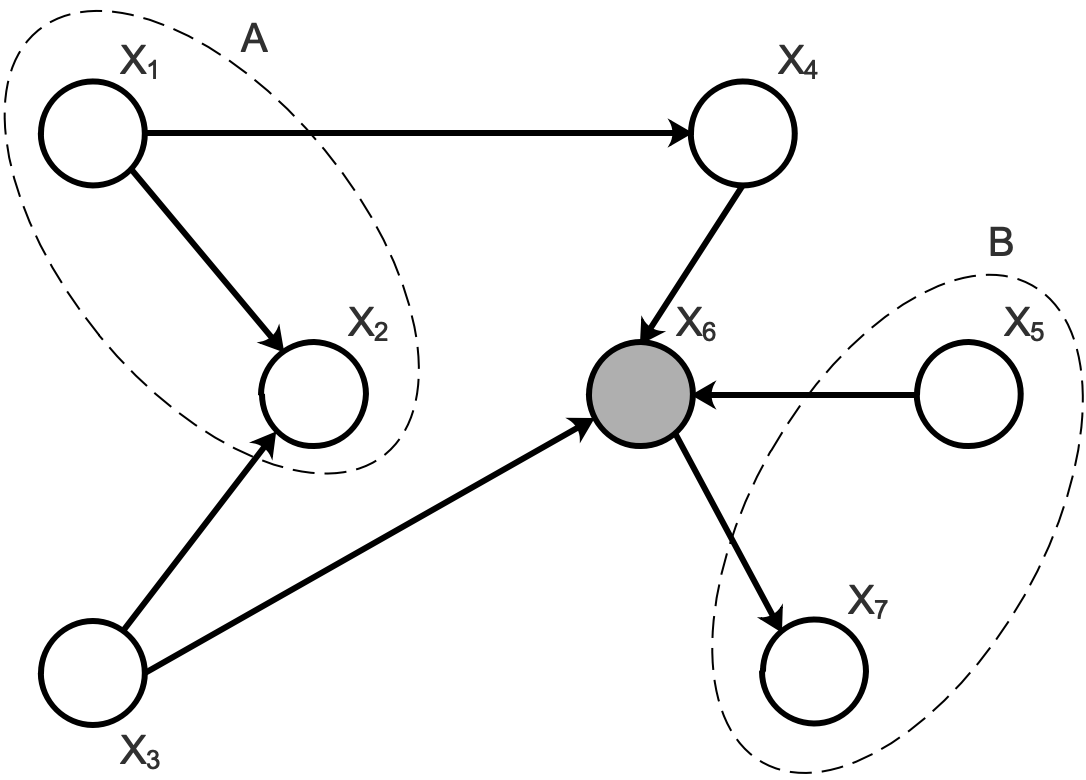
\includegraphics[width=0.7\linewidth]{dSeparationExample1_2}
\end{center}
In this case the path $X_1\rightarrow X_4\rightarrow X_6 \leftarrow X_5$ is a correct path since $X_4$ holds no evidence hence the trail $X_1\rightarrow X_4\rightarrow X_6$ is active and $X_6$ holds evidence, so the structure $X_4\rightarrow X_6\leftarrow X_5$ is active too. 
%
\subsubsection{Example 3}
Let's consider the following cases and decide whether $a$ and $b$ are d-separated:
\begin{center}
  \begin{minipage}[t]{\linewidth}
    \begin{minipage}[t]{0.48\linewidth}
      \begin{center}
        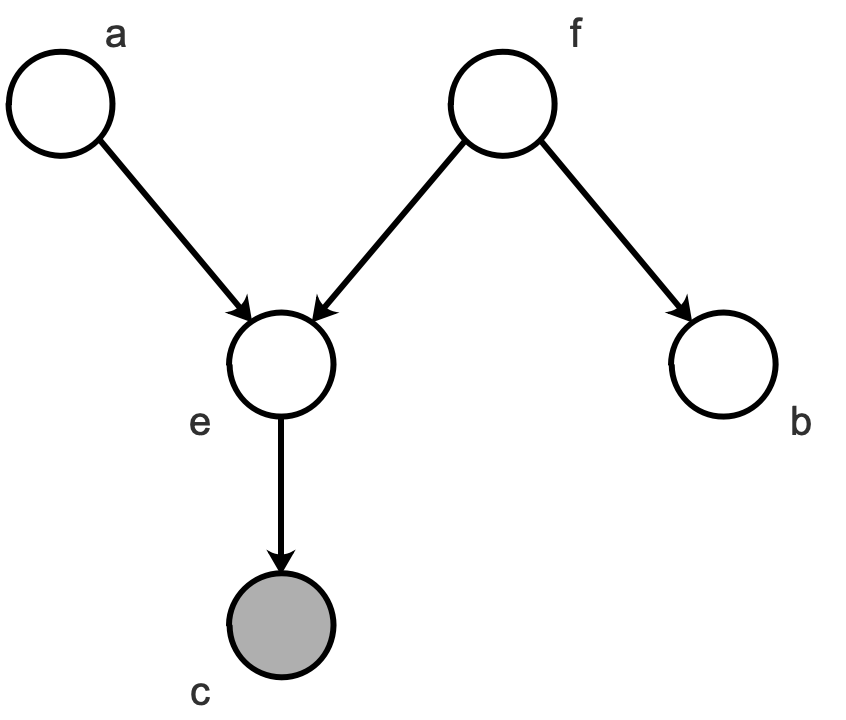
\includegraphics[width=0.8\linewidth]{dSeparationExample2_1}
      \end{center}
      In this case, the first three nodes meet a head-to-head structure and we have that $c$, which is a descendant of $e$, has evidence, hence the trail is active. The last three nodes are in a tail-to-tail structure, $f$ does not have any evidence, hence the path is valid and $a$ and $b$ are not d-separated since there exists a path from $a$ to $b$. 
    \end{minipage}
    \hspace{0.03\linewidth}
    \begin{minipage}[t]{0.48\linewidth}
      \begin{center}
        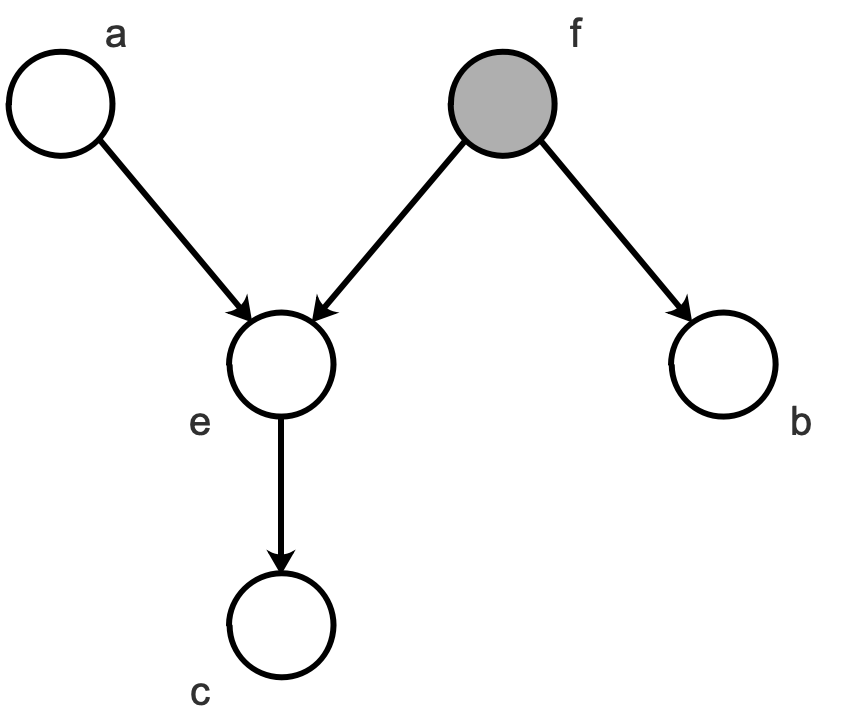
\includegraphics[width=0.8\linewidth]{dSeparationExample2_2}
      \end{center}
      It's immediate to see that $f$ is observed, hence the trail $e\leftarrow f\rightarrow b$ is not active, and also there is no evidence for $e$ or any of its descendants. By Definition~\ref{def:dSeparation}, $a$ and $b$ are d-separated given $f$: $a\perp b\vert f$.
    \end{minipage}
  \end{minipage}
\end{center}
%
%
%
\section{Bayesian Networks independences}
We saw how local independences work, that is independences between nodes, now we are going to define also global dependencies. \newline
\begin{definition}[Local Independece]
  A Bayesian Networks structure $\mathcal{G}$ encodes a set of local independence assumptions:
  \[\mathcal{I}_l(\mathcal{G})=\{\forall i~ x_i\perp \text{nondescendants}_{x_i}\vert \text{parents}_{x_i}\}\]
\end{definition}
\begin{definition}[Global Independence]
  A Bayesian Network structure $\mathcal{G}$ encodes a set of global (Markov) independence assumptions:
  \[\mathcal{I}(\mathcal{G})=\{(A\perp B\vert C):\dsep{A;B\vert C}\}\]
\end{definition}
Notice that the global independences contain the local independences.
%
%
%
\section{$l$-Equivalence}
We can notice that different structures actually encode the same set of independences assumptions. Let's consider for example head-to-head in one direction or in the other: if the intermediate node does not present evidence, then the two structures encode the same independence. In Figure~\ref{fig:lEquivalence} are shown two equivalence classes. 
\begin{figure}[htp]
  \centering
  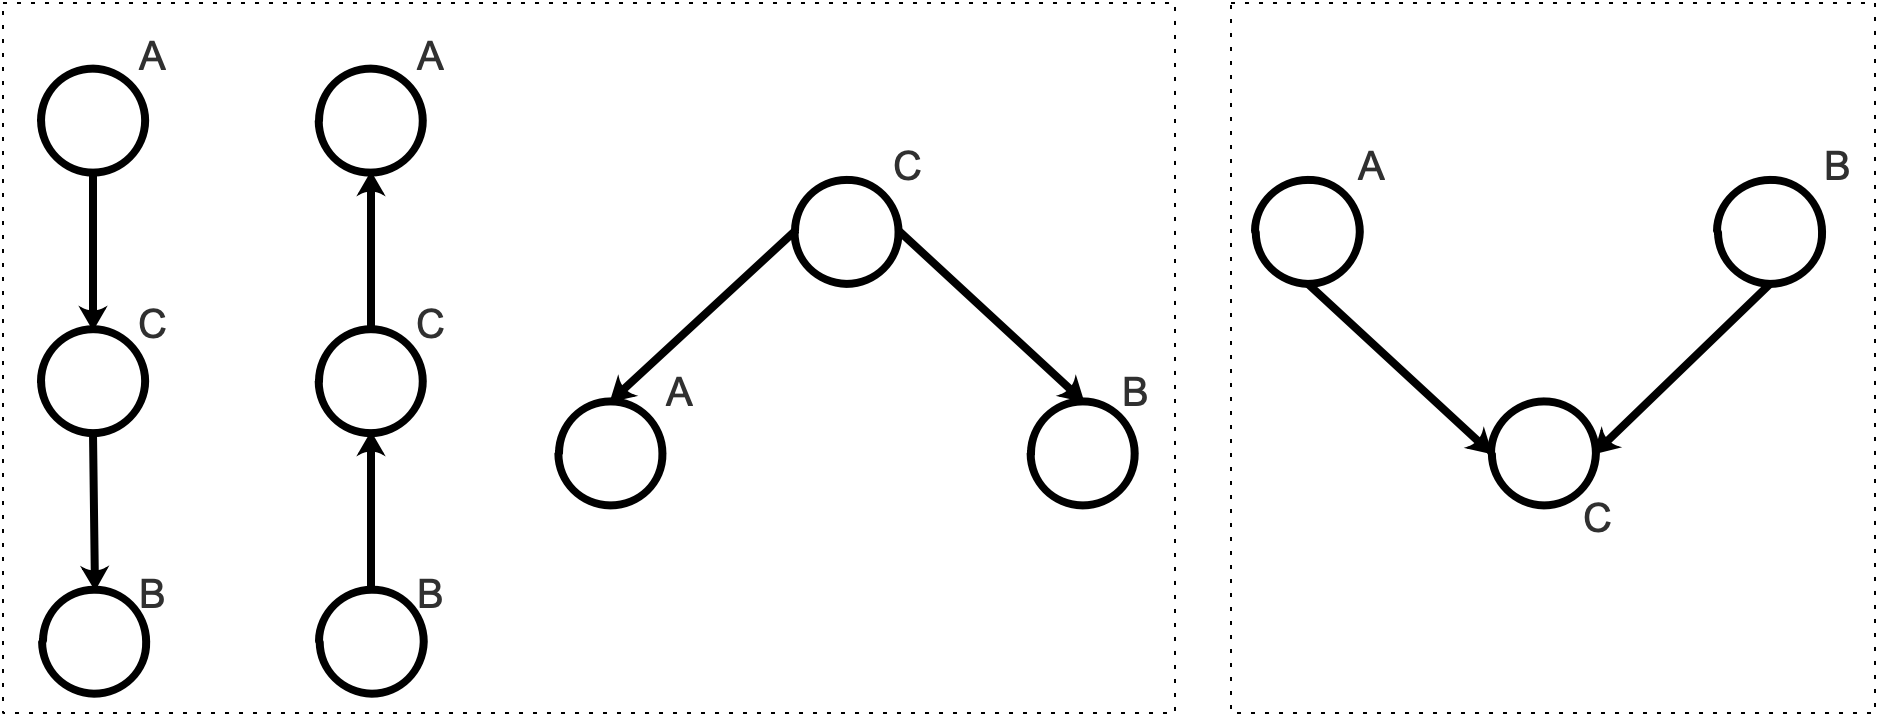
\includegraphics[width=0.8\linewidth]{lEquivalence}
  \caption{Two equivalence classes.}
  \label{fig:lEquivalence}
\end{figure}
\begin{definition}[$l$-Equivalence]
  Two Bayesian Networks structures $\mathcal{G}$ and $\mathcal{G}'$ are $l$ equivalent if $\mathcal{I}(\mathcal{G})=\mathcal{I}(\mathcal{G}')$.
\end{definition}
The space of Bayesian Network structures over the set of nodes $\mathcal{X}$ is partitioned into a set of mutually exclusive and exhaustive $l$-equivalence classes. \newline
Note that $l$-equivalence of two graphs implies that any distribution $P$ that can be factorized over on of these graphs can be factorized over the other too. Furthermore, there is no intrinsic property $P$ that would allow us to associate it with one graph rather than an equivalent one. In other words, although we can determine, for a distribution $P(X,Y)$, whether $X$ and $Y$ are correlated, there is nothing in the distribution that can help us determine whether the correct structure is $X\rightarrow Y$ or $Y\rightarrow X$. \newline
\begin{definition}[Skeleton]
  The skeleton of a Bayesian network graph $\mathcal{G}$ over a set of nodes $\mathcal{X}$ is an undirected graph over $\mathcal{X}$ that contains an edge $\{X,Y\}$ for every edge $(X,Y)$ in $\mathcal{G}$.
\end{definition}
It's possible to prove that if two structures $\mathcal{G}$ and $\mathcal{G}'$ have the same skeleton and the same set of v-structures, then they are $l$-equivalent. 
\begin{center}
  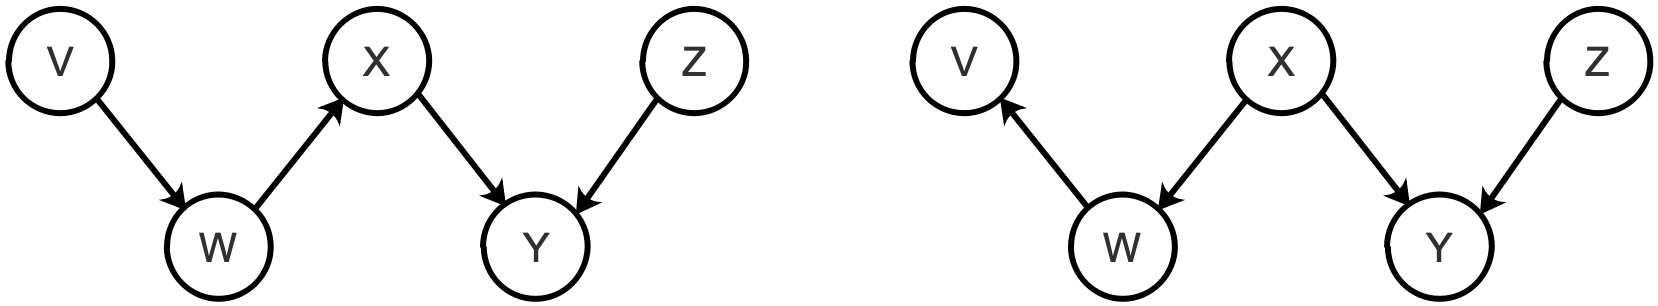
\includegraphics[width=0.7\linewidth]{lEquivalenceSkeleton}
\end{center}
Considering the above structures, they are $l$-equivalent since they have the same skeleton and the same v-structure ($X\rightarrow Y\leftarrow Z$). \newline
This is actually a \textit{sufficient condition}. Instead it's possible to have a \textit{necessary and sufficient condition} by considering also \textbf{immoralities}.
\begin{definition}[Immorality]
  A v-structure $X\rightarrow Z\leftarrow Y$ is an immorality if there is no direct edge between $X$ and $Y$. If there is such an edge, it is called a \textbf{covering edge} for the v-structure.  
\end{definition}
\begin{center}
  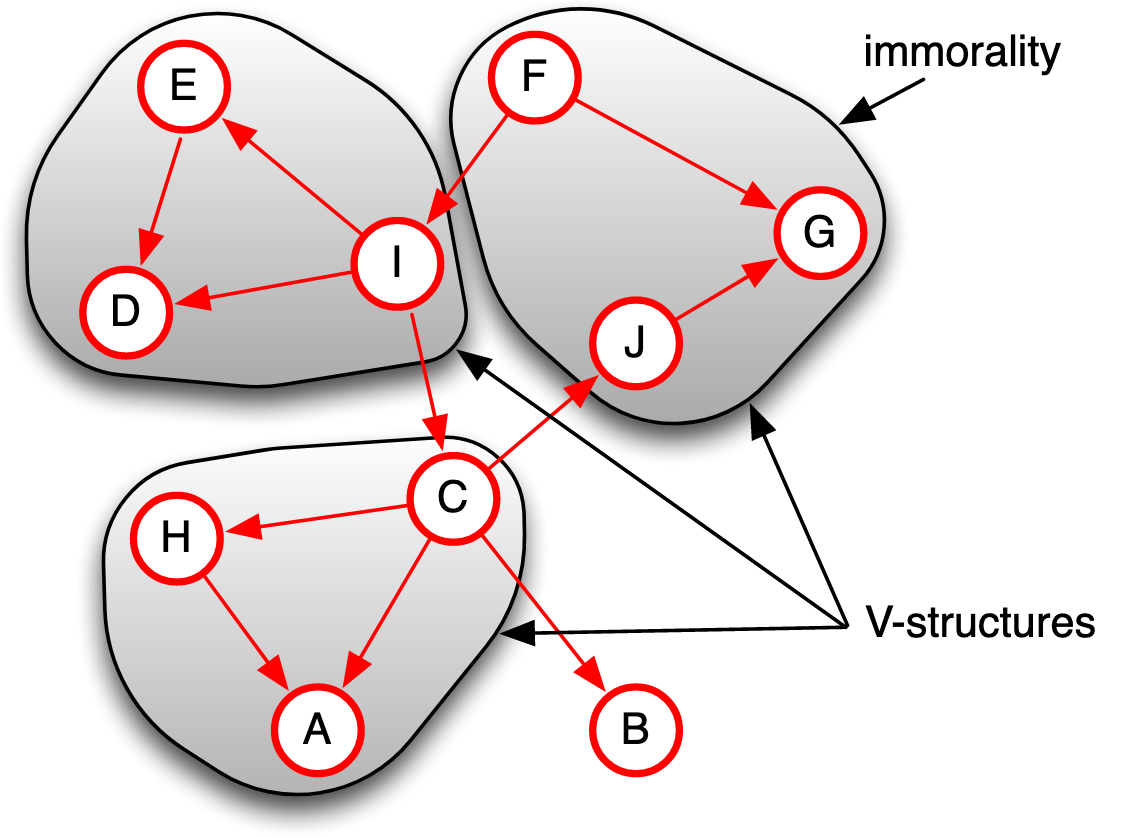
\includegraphics[width=0.6\linewidth]{lEquivalenceImmorality}
\end{center}
It's possible to notice that the v-structure $F\rightarrow G\leftarrow J$ is different from the other two since there is no edge between $F$ and $J$. This implies that such v-structure is an immorality, while the others are not immoralities. \newline
The following necessary and sufficient condition can be expressed an proven:
\begin{theorem}
  Let $\mathcal{G}_1$ and $\mathcal{G}_2$ be two graphs over a set of nodes $\mathcal{X}$. Then $\mathcal{G}_1$ and $\mathcal{G}_2$ have the same skeleton and the same set of immoralities if and only if they are $l$-equivalent. 
\end{theorem}
%
%
\subsection{$l$-Maps}
There can be two types of of maps: \textit{minimal l-maps} and \textit{P-maps}, that is perfect maps. \newline
Notice that for a structure $\mathcal{G}$ to be an $l$-map for a distribution $p$, it does not need to encode all its independences, e.g., a fully connected graph is an $l$-map of any $p$ defined over its variables.
\begin{definition}[Minimal $l$-Map]
  A minimal $l$-map for a distribution $p$ is an $l$-map $\mathcal{G}$ which can't be reduced into a $\mathcal{G}'\subset \mathcal{G}$ that is also an $l$-map for $p$.
\end{definition}
To reduce an $l$-map to another $l$-map means that by removing some edges we obtain again a valid $l$-map. \newline
Note that by this definition, a minimal $l$-map for $p$ does not necessarily capture all the independences in $p$. On the contrary a perfect $P$-map does:
\begin{definition}[$P$-Map]
  A structure $\mathcal{G}$ is a perfect map $P$-map for a distribution $p$ if it captures all (and only) its independences:
  \[\mathcal{I}(\mathcal{G})=\mathcal{I}(p)\]
\end{definition}
Notice that a $P$-map is also a minimal $l$-map, while the opposite is not valid. \newline
There exists an algorithm that allows one to find a $P$-map for a distribution $p$, but it's exponential w.r.t. the \textit{in-degree} of the $P$-map, that is the maximum number of connections of the nodes. Moreover the algorithms returns an equivalence class rather than a single structure. \newline
Moreover there are some distributions for which is not possible to find $P$-maps. In these cases, indirect graphs called Markov Networks are used.
%
%
%
\section{Making Bayesian Networks}
The first step is to find a field-expert who can tell us the variables that we may need. For example, if we are trying to develop an algorithm to predict a disease, we need to know all the possible symptoms. \newline
The next step is to actually define the variables that can be observed or that you can be interested in predicting, also latent variables can be useful. \newline
By following \textit{causality} considerations, we try to add edges to the variables. This would allow us to have a more interpretable network and also a sparser one. \newline
Lastly we start to add the probabilities for the configurations and its best to (almost) never assign zero probabilities. If any data are available, we should use them to help in learning parameters, and also the structure. 
%
%
%
\section{Inference in Graphical Models}
Bayesian Networks, as all the graphical models, actually models a joint probability. \newline
Assume we have evidence $\vect{e}$ on the state of a subset of variables $\vect{E}$ in the model. Inference amounts at computing the posterior probability of a subset $\vect{X}$ of the non-observed variables given the observations:
\[P(\vect{X}\vert\vect{E}=\vect{e})=\dfrac{P(\vect{X}, \vect{E})}{P(\vect{E}=\vect{e})}\]
The problem consists in estimating such joint probabilities when dealing with a large number of variables: directly working on the full joint probabilities would require time exponential in the number o variables. For instance, if all $N$ variables are discrete and take one of $K$ possible values, a joint probability table has $K^N$ entries. 
\[P(\vect{X}\vert\vect{E}=\vect{e})=\dfrac{P(\vect{X}, \vect{E})}{P(\vect{E}=\vect{e})}=\Sum_{Y_1,\hdots,Y_n}P(\vect{X},Y_1,\hdots,Y_n,\vect{E}=\vect{e})\]
Our goal is to exploit the structure in graphical models to do inference more efficiently.
%
%
\subsection{Inference -- Chain}
The most simple structure we have seen is a chain of nodes where each variable has a connection to the following one. 
\begin{center}
  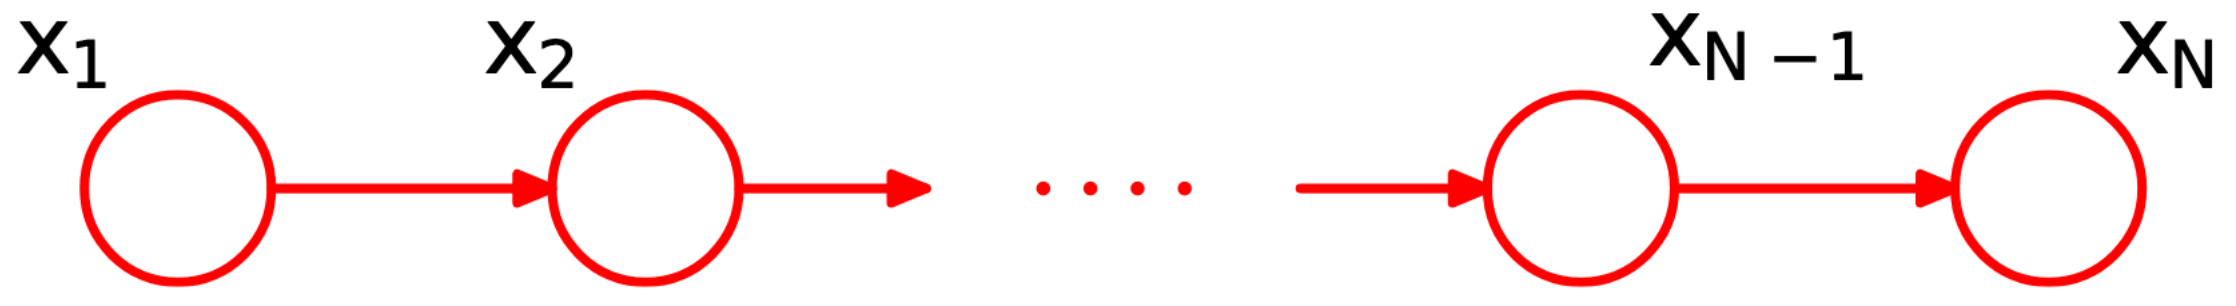
\includegraphics[width=0.7\linewidth]{InferenceChain}
\end{center}
In this way the probability of all variables in the chain becomes:
\[P(X)=P(X_1)\cdot P(X_2\vert X_1)\cdot \hdots \cdot P(X_{N}\vert X_{N-1})\]
The marginal probability of an arbitrary variable $X_i$ is:
\[P(X_i)=\Sum_{X_1}\Sum_{X_2}\hdots \Sum_{X_{i-1}}\Sum_{X_{i+1}}\hdots\Sum_{X_n}P(\vect{X})\]
Suppose that $i=N$, then it's possible to see that only $P(X_N\vert X_{N-1})$ is involved in the last summation which can be computed first giving a function of $X_{N-1}$:
\[\mu_\beta(X_{N-1})-=\Sum_{X_N}P(X_N\vert X_{N-1})\]
Noe let's suppose that $i=N-1$, then the marginalization can be iterated as:
\[\mu_\beta(X_{N-1})=\Sum_{X_{N-1}}P(X_{N-1}\vert X_{N-2})\mu_\beta(X_{N-1})\]
One could decrease the value of $i$ and obtain the general function:
\[\mu_\beta(X_i)=\Sum_{X_{i+1}}P(X_{i+1}\vert X_{i})\mu_\beta(X_{i+1})\]
Now let's try to do the opposite and start from the front: 
\[\mu_\alpha(X_2)=\Sum_{X_1}P(X_1)P(X_2\vert X_1)\]
\[\mu_\alpha(x_3)=\Sum_{x_2}P(x_3\vert x_2)\mu_\alpha(x_2)\]
It's possible to see the marginalization of the chain as a product of $\mu_\alpha$ and $\mu_\beta$. Indeed, we could write:
\[P(X_i)=\mu_\alpha(X_i)\mu_\beta(X_i)\]
We could think of $\mu_\alpha(X_i)$ and $\mu_\beta(X_i)$ as messages passing from $X_{i-1}$ to $X_{i}$ and from $X_{i+1}$ to $X_i$ respectively\footnote{$\alpha$ is passing the message forward, $\beta$ is passing the message backwards.}:
\[\mu_\alpha=\Sum_{X_{i-1}}P(X_i\vert X_{i-1})\mu_\alpha(X_{i-1})\]
\[\mu_\beta=\Sum_{X_{i+1}}P(X_{i+1}\vert X_{i})\mu_\beta(X_{i+1})\]
%TODO add image here of message passing
Each outgoing message is obtained by multiplying the incoming message by the local probability and summing over the node values. 
Suppose we want to compute the marginal probabilities for a number of different variables $\vect{X}_i$. For each variable we should send a message from the beginning to the variable and from the variable to the end of the chain. Since the probabilities at each node is not going to change, then one could simply send a message from the beginning to the end and one from the end to the beginning. If all nodes store messages, we can compute any marginal probability as:
\[P(\vect{X}_i)=\mu_\alpha(\vect{X}_i)\mu_\beta(\vect{X}_i)\]
This does not count for evidence. If we were to consider also the case in which some nodes $\vect{X}_e$ are observed, then the formula would change and instead of summing over all possible values, we'd just use the observed values. For instance, let's consider the case in which we have 4 variables: $\vect{X}=\{X_1,X_2,X_3,X_4\}$, we could compute the probability of $\vect{X}$ as:
\[P(\vect{X})=P(X_1)P(X_2\vert X_1)P(X_3\vert X_2)P(X_4\vert X_3)\]
The marginal probability of $X_2$ and observations $X_1=x_{e_1}, X_3=x_{e_3}$ is:
\[P(X_2,X_1=x_{e_1},X_3=x_{e_3})=\Sum_{X_1}\Sum_{X_3}\Sum_{X_4}P(\vect{X})\]
\[P(X_2,X_1=x_{e_1},X_3=x_{e_3})=\Sum_{X_1}\Sum_{X_3}\Sum_{X_4}P(X_1)P(X_2\vert X_1)P(X_3\vert X_2)P(X_4\vert X_3)\]
Since $X_1=x_{e_1}$ and $X_3=x_{e_3}$, we have:
\[P(X_2,X_1=x_{e_1},X_3=x_{e_3})=P(X_1=x_{e_1})P(X_2\vert X_1=x_{e_1})P(X_3=x_{e_3}\vert X_2)\Sum_{X_4}P(X_4\vert X_3=x_{e_3})\]
Whne adding evidence, the message passing procedure computes the joint probability of the variable and the evidence, hence it has to be normalized to obtain the conditional probability given the evidence:
\[P(X_n\vert \vect{X}_e=\vect{x}_e)=\dfrac{P(X_n, \vect{X}_e=\vect{x}_e)}{\Sum_{X_n}P(X_n,\vect{X}_e=\vect{x}_e)}\]
%
%
\subsection{Inference -- Trees}
Obviously chains are not the only existing structure, but trees are another type of structure. In this case we can consider three cases:
\begin{itemize}
  \item \textbf{Undirected trees}: undirected graphs with a single path for each pair of nodes.
  \item \textbf{Directed trees}: directed graphs with a single node with no parentes (root) and all the other nodes with a single parent.
  \item \textbf{Directed polytrees}: directed graphs with multiple parents for node and multiple roots, but still a single (undirected) path between each pair of nodes. 
\end{itemize}
\begin{minipage}[htp]{\linewidth}
  \begin{center}
    \begin{minipage}{0.3\linewidth}
      \begin{center}
        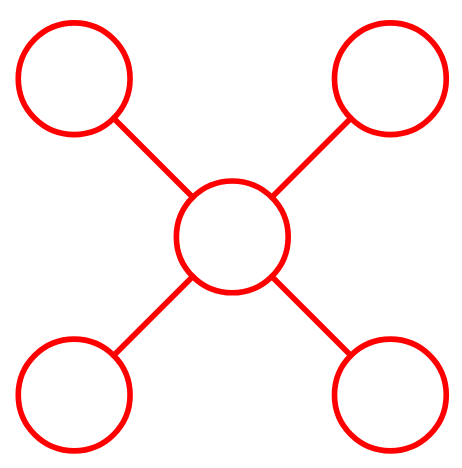
\includegraphics[height=3.5cm]{InferenceTrees1}\\
        Undirected trees.
      \end{center}
    \end{minipage}
    \hspace{0.01\linewidth}
    \begin{minipage}{0.3\linewidth}
      \begin{center}
        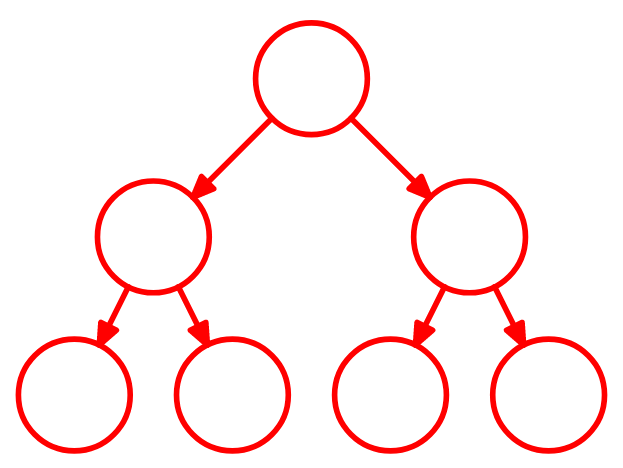
\includegraphics[width=\linewidth]{InferenceTrees2}\\
        Directed trees.
      \end{center}
    \end{minipage}
    \hspace{0.01\linewidth}
    \begin{minipage}{0.3\linewidth}
      \begin{center}
        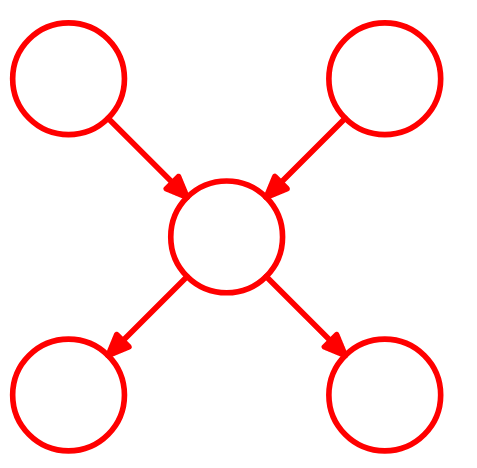
\includegraphics[height=3.5cm]{InferenceTrees3}\\
        Directed polytrees.    
      \end{center}
    \end{minipage}
  \end{center}
\end{minipage}\\
\vspace{0.3cm}
Since explaining these structures per se is quite troublesome, we are introducing \textbf{facto graphs}.
%
%
\subsection{Inference -- Factor Graph}
Factor graphs are an alternative graphical representation which is useful to better explain inference algorithms. \newline
A factor graph is a graphical representation of a graphical model highlighting its factorization, i.e., its conditional probabilities. A factor graph has one node for each node in the original graph, one additional node for each factor (evidence) and undirected links to each of the node variables in the factor. \newline
Mind that each node factor needs to be linked to all the nodes from which the decomposition comes from. \newline
Let's consider for example the following probability distribution:
\[P(X_3\vert X_1,X_2)P(X_1)P(X_2)\]
We know that a Bayesian Network representation can be:
\begin{center}
  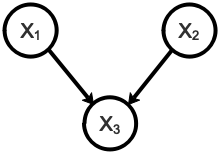
\includegraphics[scale=0.3]{FactorGraphExample1_1}
\end{center}
We could notice that actually $X_3$ is conditioned on $X_1$ and $X_2$ and hence we could create a factor node $f$ as follows:
\begin{center}
  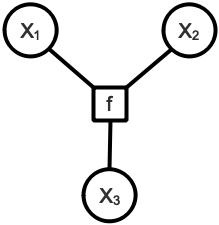
\includegraphics[scale=0.3]{FactorGraphExample1_2}
\end{center}
Actually $f$ can be thought as a function:
\[f(X_1,X_2,X_3)=P(X_3\vert X_1,X_2)P(X_1)P(X_2)\]
Now then it's possible to add also other two factor nodes which would express the probability of the nodes $X_1$ and $X_2$. 
\[f_c(X_1,X_2,X_3)=P(X_3\vert X_1,X_2)\]
\[f_a(X_1)=P(X_1)\]
\[f_b(X_2)=P(X_2)\]
\begin{center}
  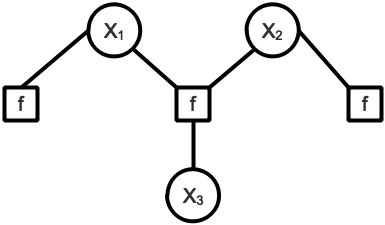
\includegraphics[scale=0.3]{FactorGraphExample1_3}
\end{center}
%
%
\subsection{Sum-Product Algorithm}
The sum-product algorithm is an efficient algorithm for exact inference on tree-structured graphs. As the version for the chains, also this is a message passing algorithm. \newline
This algorithm is applicable to undirected models, i.e., Markov Networks, as well as directed ones, i.e., Bayesian Networks. 
We will now present it on factor graphs assuming a tree-structured graph giving rise to a factor graph which is a tree. \newline
%
\subsubsection{Computing Marginals}
To compute the probability of a single variable, one sums over the probabilities of all variables except the one for which they wish to compute the marginal. \newline
\[P(X)=\Sum_{\vect{X}\setminus X}P(\vect{X})\]
Since $X$ is a node, then the probability $P(X)$ of an event is the product of all the incoming messages from the neighbouring factors $f_s$:
\[P(X)=\Prod_{f_s\in \neigh(X)}\mu_{f_s\rightarrow X}(X)\]
where $\neigh(X)$ are the neighbours of $X$.


Dato un nodo $x_i$, possiamo scrivere il messaggio in uscita $\mu_{\alpha}(x_{i+1})$ come:
\[\mu_{\alpha}(x+1)=\Sum_{X_i}P(x_{i+1}\vert x_i)\mu_\alpha(x_i)\]
Quindi possiamo scrivere il messaggio $\mu_{f_i\rightarrow x}(x)$ come: 
\[ \mu_{f\rightarrow x}(x)=\Sum_{x_i...x_m}f(x_1, ..., x_m)\Pi_{x_f\in}\]
Possiamo vedere che sia se il messaggio è da un factor a un nodo, sia che il messaggio sia da un nodo a un factor, si tratta comunque di una funzione del nodo. \newline 
vedi fogli che forse si capisce qualcosa di più


